% Modelo C4 do ViaJá
% Para usar no Overleaf: envie este arquivo junto com a pasta img/ e compile com pdfLaTeX.
\documentclass[12pt,a4paper]{article}

\usepackage[utf8]{inputenc}
\usepackage[T1]{fontenc}
\usepackage[brazilian]{babel}
\usepackage[a4paper,margin=2.5cm]{geometry}
\usepackage{graphicx}
\usepackage{booktabs}
\usepackage{tabularx}
\usepackage{array}
\usepackage{float}
\usepackage{xcolor}
\usepackage{caption}
\usepackage{enumitem}
\usepackage[hidelinks]{hyperref}

\graphicspath{{img/}}
\definecolor{viaja}{HTML}{1F3A5F}
\captionsetup{font=small,labelfont=bf}
\renewcommand{\arraystretch}{1.25}
\newcolumntype{L}{>{\raggedright\arraybackslash}X}
\newcommand{\classe}[1]{\texttt{#1}}

\begin{document}

% ---------------------------------------------------------------- capa
\begin{titlepage}
    \centering
    {\large\bfseries\color{viaja} Universidade Católica do Salvador (UCSAL)\par}
    {\large\color{viaja} Escola de Tecnologias \textperiodcentered{} Engenharia de Software\par}
    \vspace{0.6cm}
    {\normalsize Disciplina: Tópicos Avançados em Programação\par}
    \vfill
    {\Huge\bfseries\color{viaja} Sistema ViaJá\par}
    \vspace{0.6cm}
    {\Large Plataforma de Reserva de Passagens, Hospedagem e Itinerários\par}
    \vspace{0.4cm}
    {\Large\bfseries Modelo C4\par}
    {\large Contexto, Contêineres, Componentes e Código\par}
    \vfill
    {\small\bfseries EQUIPE\par}
    \vspace{0.2cm}
    Abraão\par
    Guilherme\par
    João Pedro\par
    Lucca (ScrumMaster)\par
    William\par
    \vspace{0.6cm}
    {\small\bfseries PROFESSOR\par}
    \vspace{0.2cm}
    Elton Figueiredo da Silva\par
    \vfill
    Salvador, BA \textperiodcentered{} Novembro de 2026\par
\end{titlepage}

\tableofcontents
\newpage

% ---------------------------------------------------------------- introdução
\section{Introdução}

Este documento descreve a arquitetura do ViaJá com o modelo C4, que apresenta um sistema em quatro
níveis de detalhe. Cada nível responde a uma pergunta:

\begin{enumerate}[leftmargin=*]
    \item \textbf{Contexto:} quem usa o sistema e com quais sistemas externos ele conversa?
    \item \textbf{Contêineres:} quais são as partes que rodam separadas e como se comunicam?
    \item \textbf{Componentes:} o que existe dentro da API e qual a responsabilidade de cada parte?
    \item \textbf{Código:} como as classes mais importantes se relacionam?
\end{enumerate}

O ViaJá é uma plataforma web que reúne busca de passagens, hospedagens e passeios, montagem de
itinerário com validação de datas, um assistente de roteiro com IA e a solicitação de reserva sem
pagamento. O back-end é escrito em Java com Spring Boot, o front-end em React e o banco de dados é um
H2 em memória, embutido na própria API.

Nos diagramas, as cores seguem a convenção do C4: azul-escuro para pessoas, azul para o sistema e
seus contêineres, azul-claro para componentes e cinza para sistemas externos. Os diagramas são
escritos em Mermaid e ficam versionados no repositório, na pasta \texttt{docs/c4}.

% ---------------------------------------------------------------- nível 1
\section{Nível 1: Contexto}

O diagrama de contexto mostra o ViaJá como uma caixa única, os três perfis de usuário e os dois
sistemas externos de que ele depende.

\begin{figure}[H]
    \centering
    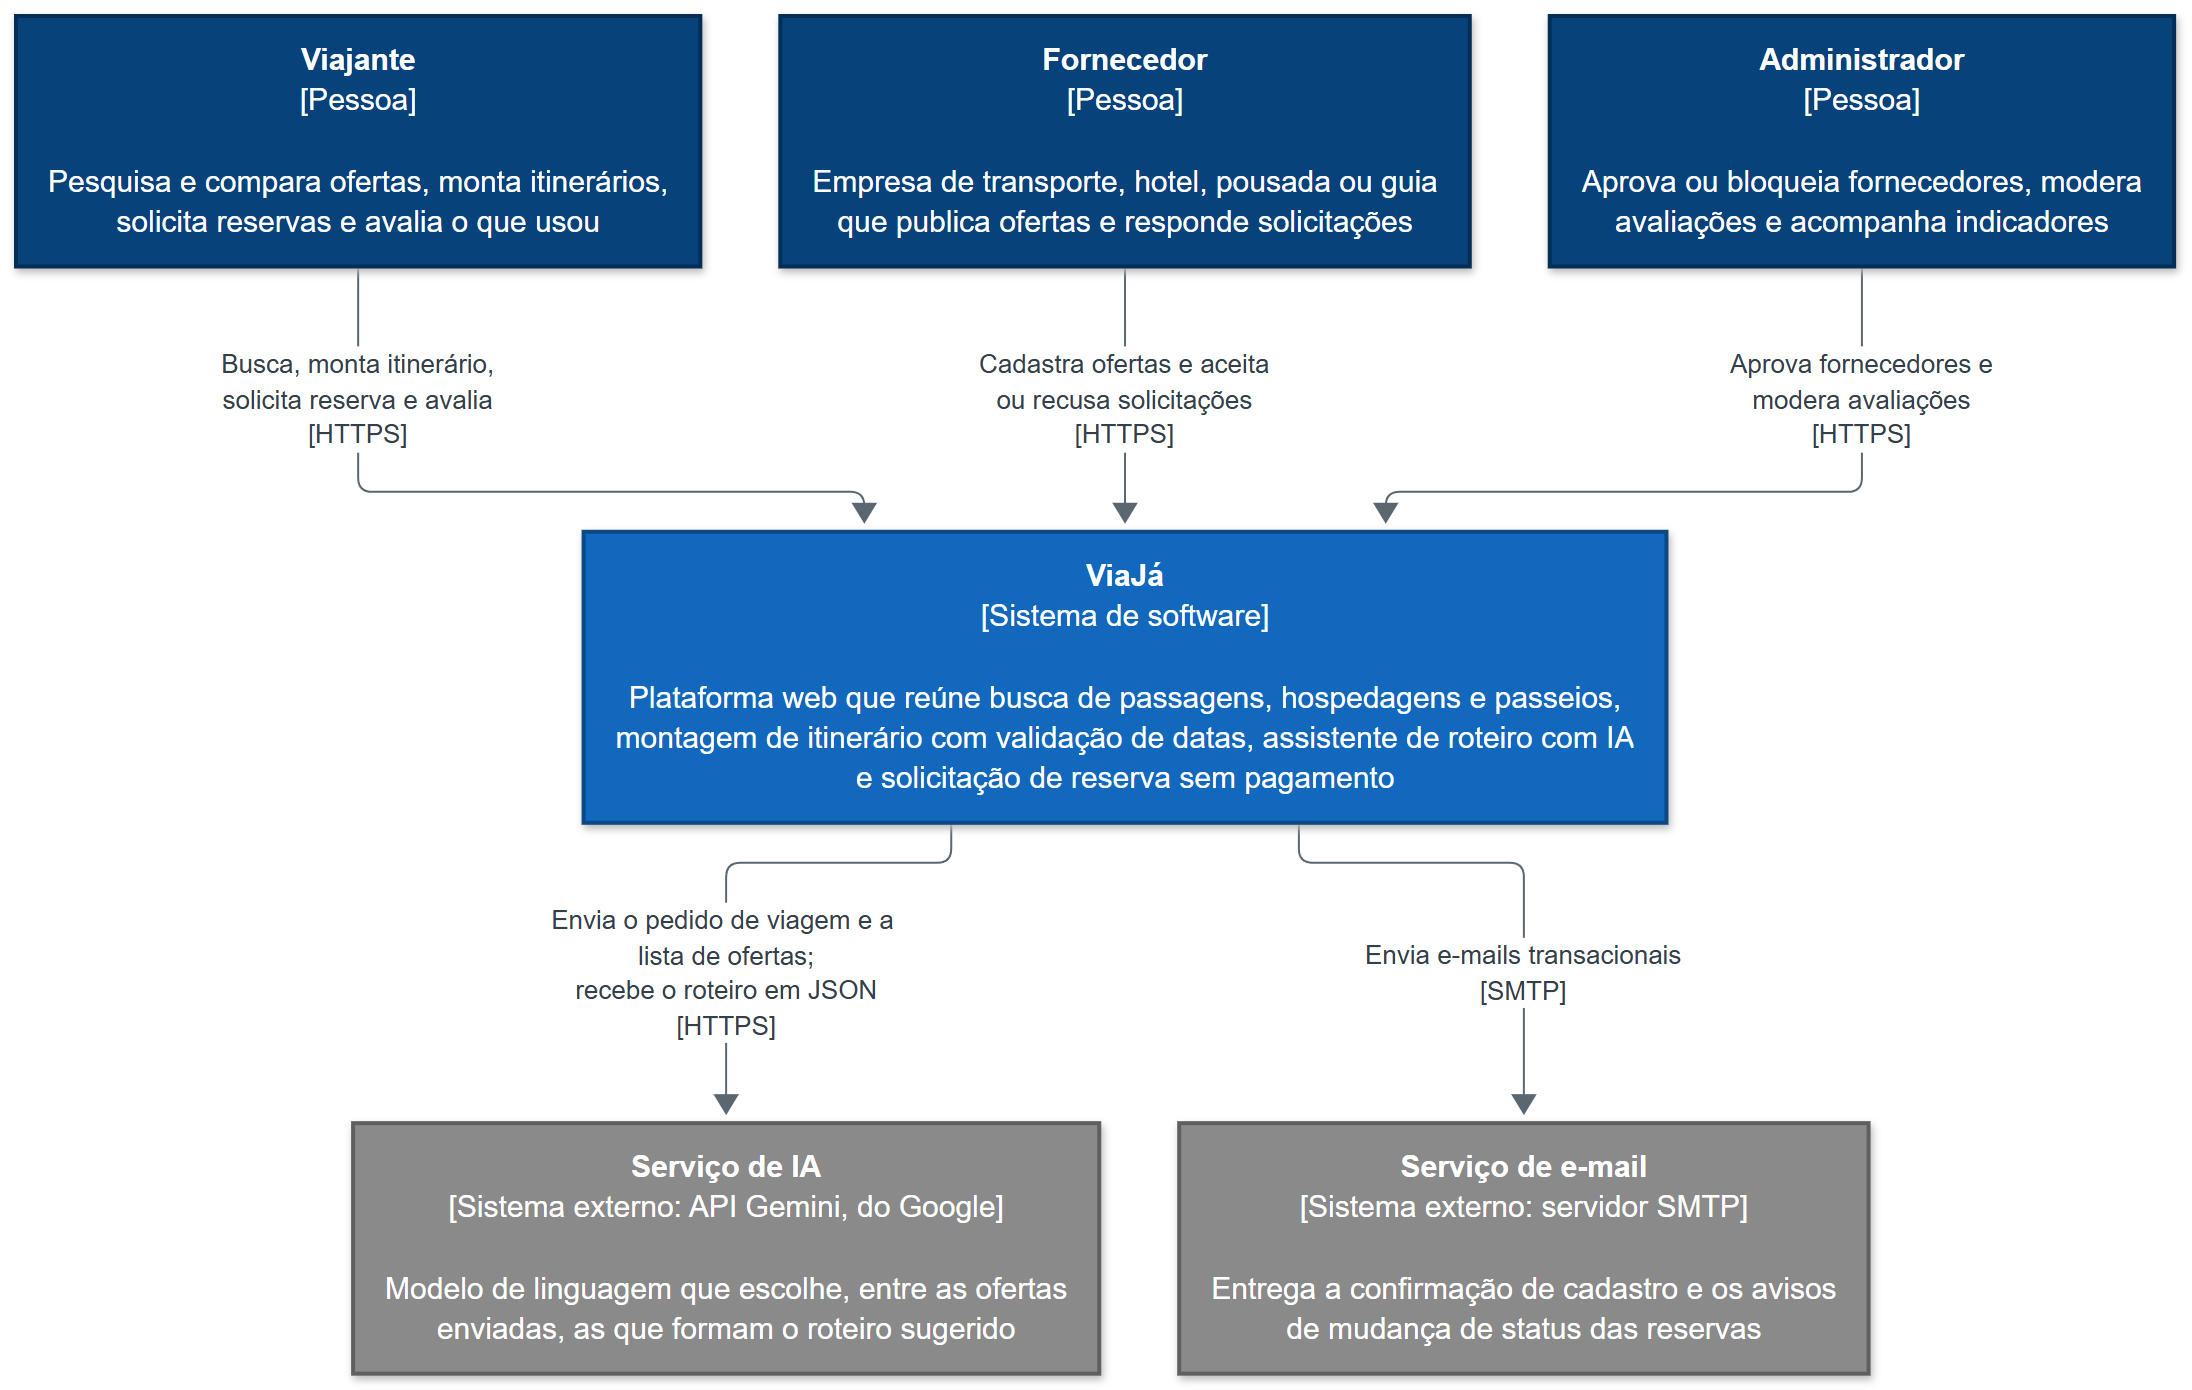
\includegraphics[width=\linewidth]{c4-1-contexto.png}
    \caption{Diagrama de contexto do ViaJá.}
\end{figure}

\begin{table}[H]
    \small
    \begin{tabularx}{\linewidth}{@{}p{3.2cm}p{2.6cm}L@{}}
        \toprule
        \textbf{Elemento} & \textbf{Tipo} & \textbf{Papel} \\
        \midrule
        Viajante & Pessoa & Pesquisa e compara ofertas, monta itinerários, usa o assistente de IA, solicita reservas e avalia o que usou. \\
        Fornecedor & Pessoa & Empresa de transporte, hotel, pousada ou guia local. Publica ofertas e aceita ou recusa solicitações. \\
        Administrador & Pessoa & Aprova ou bloqueia fornecedores, modera avaliações e acompanha indicadores de uso. \\
        ViaJá & Sistema & Plataforma web de busca, itinerário e solicitação de reserva sem pagamento. \\
        Serviço de IA & Sistema externo & API Gemini, do Google. Recebe o pedido de viagem e a lista de ofertas e devolve o roteiro em JSON. \\
        Serviço de e-mail & Sistema externo & Servidor SMTP que entrega a confirmação de cadastro e os avisos de reserva. \\
        \bottomrule
    \end{tabularx}
    \caption{Elementos do diagrama de contexto.}
\end{table}

Ficam fora do contexto, de propósito, os itens cortados do MVP: gateway de pagamento, emissão de
bilhetes e integração com companhias aéreas ou redes hoteleiras.

% ---------------------------------------------------------------- nível 2
\section{Nível 2: Contêineres}

O diagrama de contêineres abre a caixa do ViaJá e mostra as três partes que rodam separadas.

\begin{figure}[H]
    \centering
    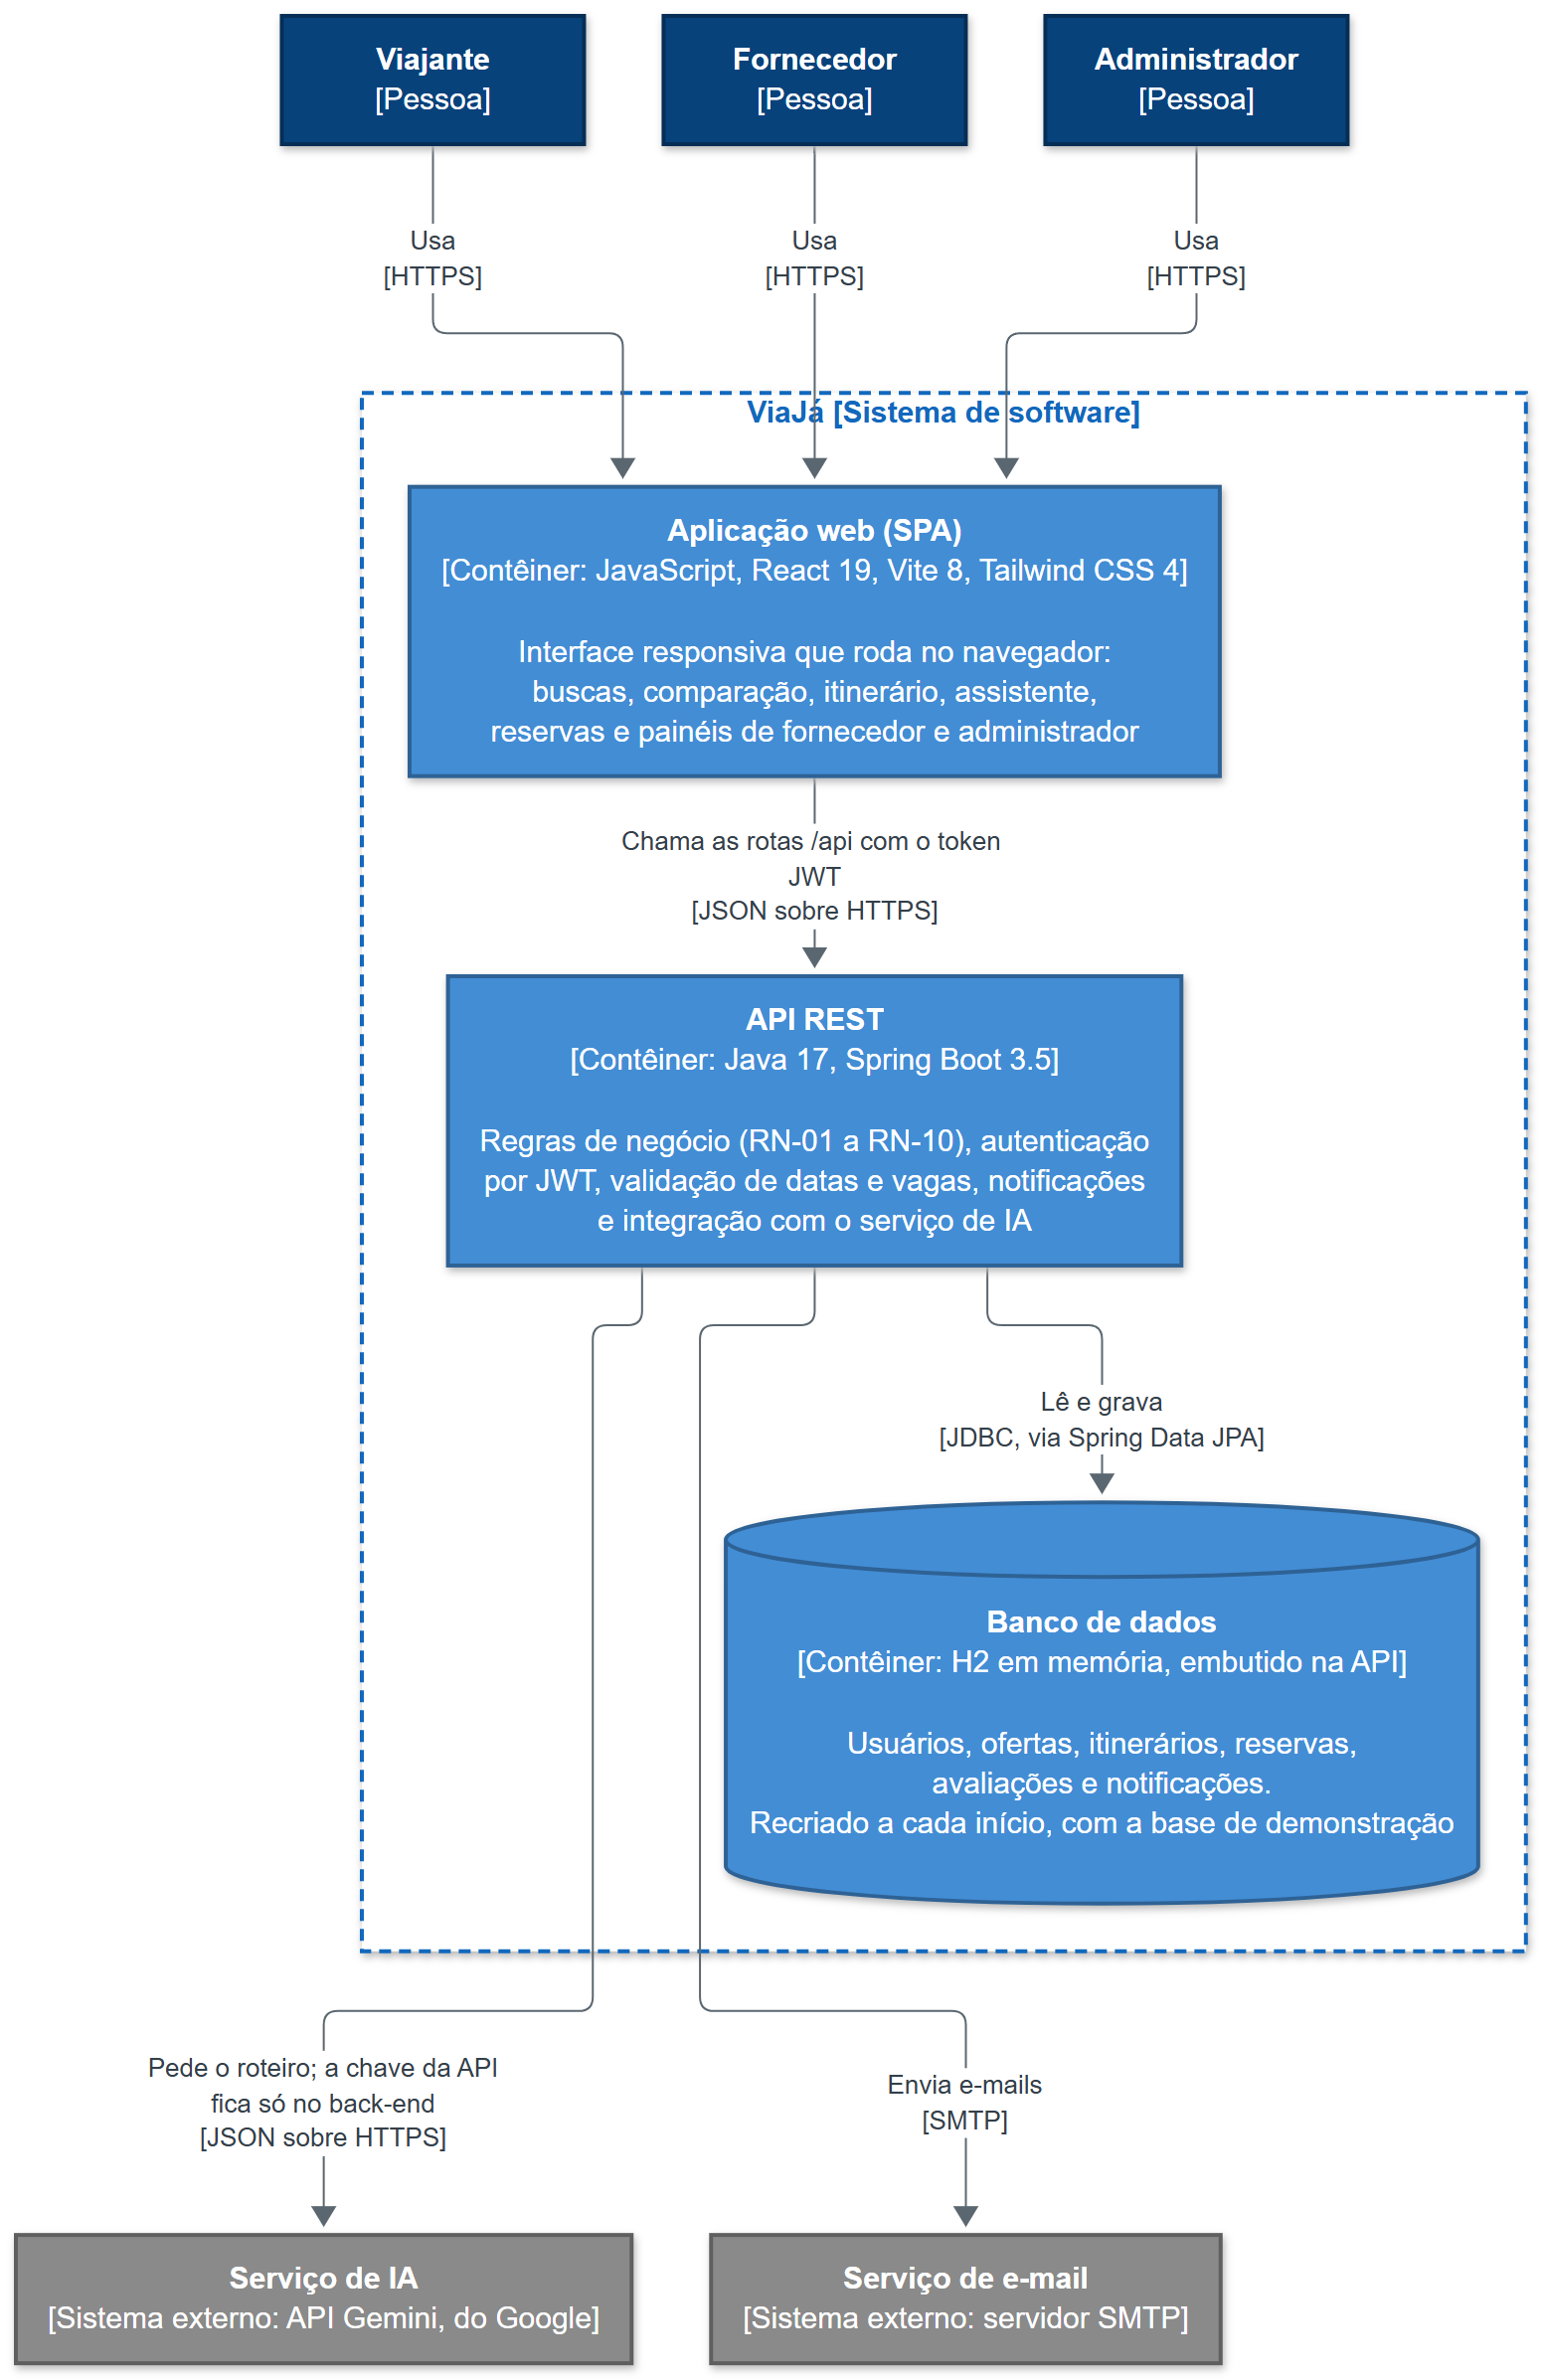
\includegraphics[width=0.78\linewidth,height=0.62\textheight,keepaspectratio]{c4-2-conteineres.png}
    \caption{Diagrama de contêineres do ViaJá.}
\end{figure}

\begin{table}[H]
    \small
    \begin{tabularx}{\linewidth}{@{}p{3.2cm}p{4.2cm}L@{}}
        \toprule
        \textbf{Contêiner} & \textbf{Tecnologia} & \textbf{Responsabilidade} \\
        \midrule
        Aplicação web (SPA) & JavaScript, React 19, Vite 8, Tailwind CSS 4 & Interface responsiva que roda no navegador. Não guarda regra de negócio nem segredo. \\
        API REST & Java 17, Spring Boot 3.5, Spring Security, Spring Data JPA & Regras de negócio, autenticação por JWT, validação de datas e vagas, notificações e chamada ao serviço de IA. \\
        Banco de dados & H2 em memória, embutido na API & Usuários, ofertas, itinerários, reservas, avaliações e notificações. \\
        \bottomrule
    \end{tabularx}
    \caption{Contêineres do ViaJá.}
\end{table}

Decisões de arquitetura visíveis neste nível:

\begin{itemize}[leftmargin=*]
    \item \textbf{A SPA só fala com a API.} O navegador nunca acessa o banco nem o serviço de IA, e por
          isso a chave da API de IA fica apenas no back-end, em variável de ambiente (RNF-05).
    \item \textbf{Sessão sem estado.} Depois do login, a SPA envia o token JWT, válido por 24 horas, no
          cabeçalho \texttt{Authorization} de cada chamada (RNF-03).
    \item \textbf{Banco em memória.} O H2 roda dentro do processo da API, sem instalação. Os dados
          existem enquanto a API está no ar e a base de demonstração é recriada a cada início, o que
          deixa a apresentação sempre no mesmo ponto de partida. O acesso passa só pelos repositórios
          JPA, então trocar por um banco em servidor muda a configuração, e não o código.
    \item \textbf{IA com modelo reserva.} A API chama o Gemini por HTTPS com limite total de 15
          segundos (RNF-02). Se o primeiro modelo estiver sobrecarregado, tenta o seguinte; se nenhum
          responder, devolve o roteiro padrão.
\end{itemize}

% ---------------------------------------------------------------- nível 3
\section{Nível 3: Componentes}

O diagrama de componentes detalha o contêiner \textbf{API REST}. Cada componente corresponde a um
conjunto de classes do pacote \texttt{br.ucsal.viaja}.

\begin{figure}[H]
    \centering
    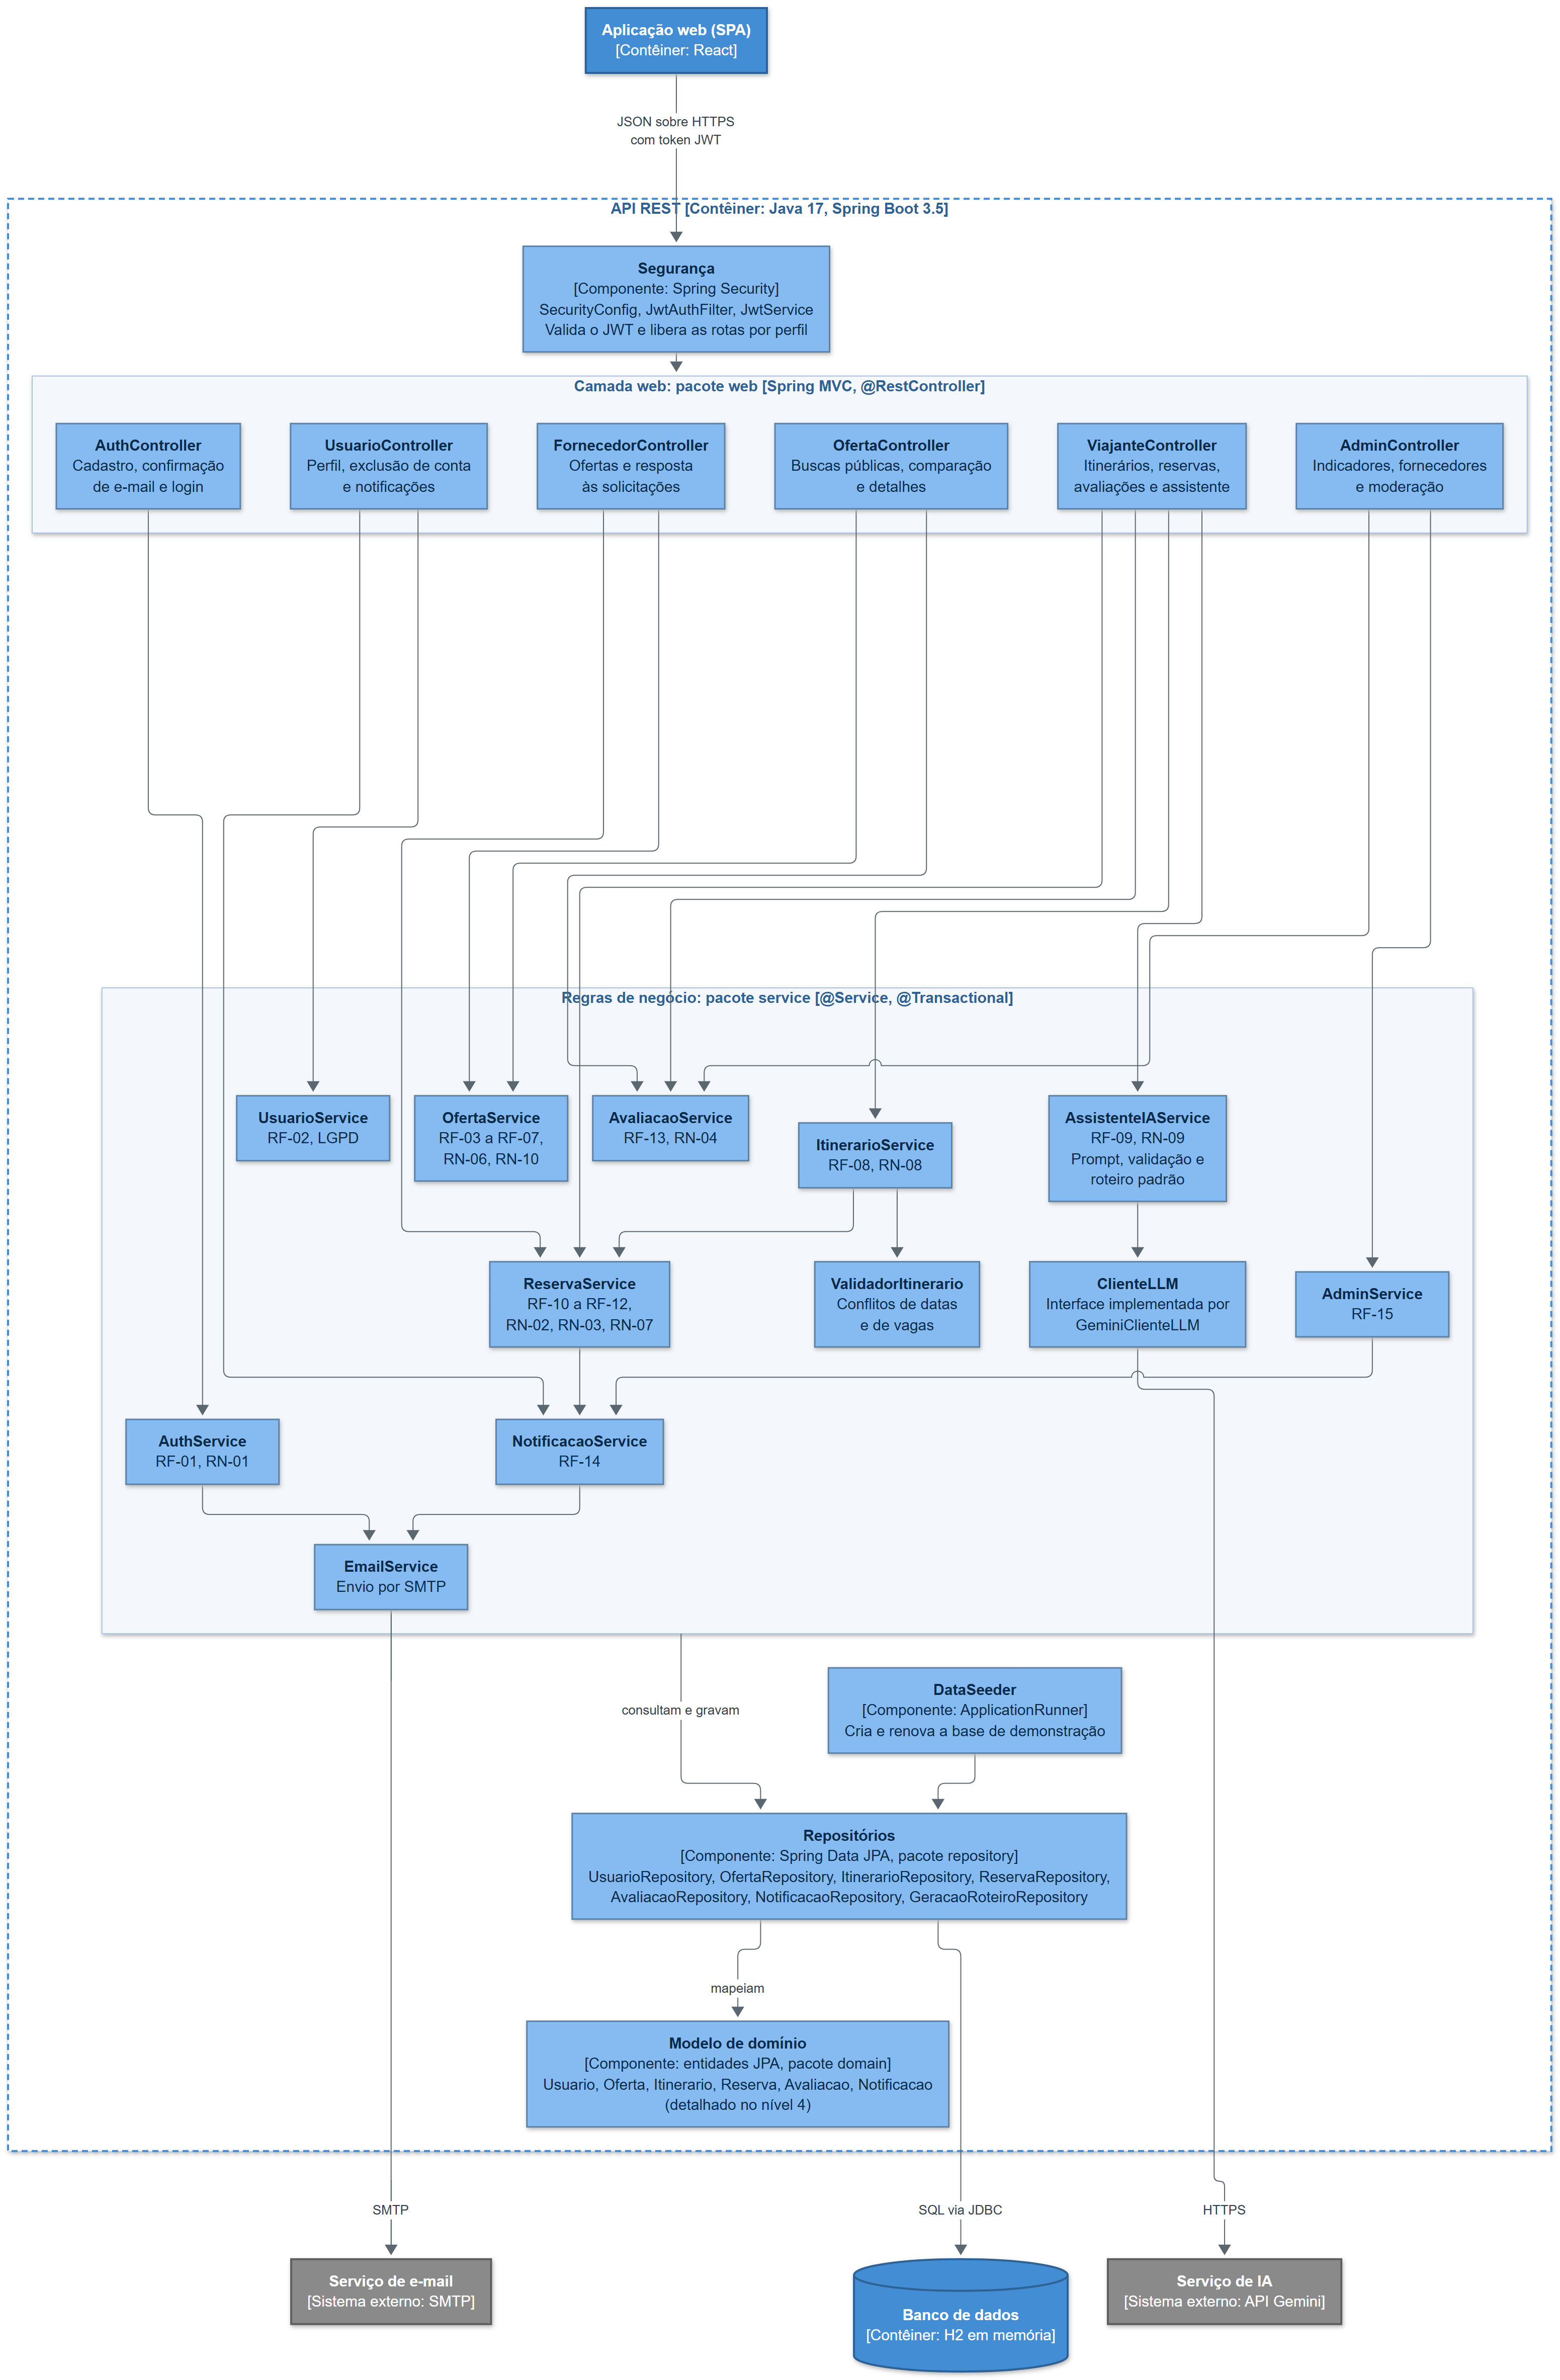
\includegraphics[width=\linewidth,height=0.86\textheight,keepaspectratio]{c4-3-componentes.png}
    \caption{Diagrama de componentes da API REST.}
\end{figure}

\begin{table}[H]
    \footnotesize
    \begin{tabularx}{\linewidth}{@{}p{4.4cm}Lp{3.1cm}@{}}
        \toprule
        \textbf{Componente} & \textbf{Responsabilidade} & \textbf{Requisitos} \\
        \midrule
        Segurança (\classe{SecurityConfig}, \classe{JwtAuthFilter}, \classe{JwtService}) & Valida o JWT, identifica o perfil e libera as rotas por perfil. Senhas com bcrypt. & RNF-03 \\
        Camada web (seis controllers e \classe{ApiExceptionHandler}) & Recebe as requisições HTTP, valida o formato dos dados e devolve JSON. & Todos os RF \\
        \classe{AuthService} & Cadastro com confirmação de e-mail e login. & RF-01, RN-01 \\
        \classe{UsuarioService} & Edição de perfil e exclusão da conta com remoção dos dados pessoais. & RF-02, RNF-04 \\
        \classe{OfertaService} & Buscas com filtros, comparação e cadastro de ofertas. & RF-03 a RF-07, RN-05, RN-06, RN-10 \\
        \classe{ItinerarioService} e \classe{ValidadorItinerario} & Itinerário por dia, custo total e conflitos de datas e de vagas. & RF-08, RN-08 \\
        \classe{ReservaService} & Solicitação, aceite, recusa, cancelamento, expiração em 48 horas e lembrete. & RF-10 a RF-12, RN-02, RN-03, RN-07 \\
        \classe{AvaliacaoService} & Avaliação de itens usufruídos e cálculo da nota média. & RF-13, RN-04 \\
        \classe{NotificacaoService} e \classe{EmailService} & Aviso dentro do sistema e por e-mail a cada mudança de status. & RF-14 \\
        \classe{AdminService} & Indicadores de uso e aprovação ou bloqueio de fornecedores. & RF-15 \\
        \classe{AssistenteIAService} & Monta o prompt, chama o modelo, valida a resposta e aplica o roteiro padrão se a IA falhar. & RF-09, RN-09, RNF-02 \\
        \classe{ClienteLLM} (\classe{GeminiClienteLLM}) & Interface de saída para o serviço de IA. A implementação chama a API Gemini por HTTPS, com limite de 15 segundos e modelo reserva. & RNF-02, RNF-05 \\
        Repositórios (Spring Data JPA) & Consultas e gravação no banco de dados. & \\
        Modelo de domínio & Entidades e regras que pertencem aos próprios objetos. & RN-01 a RN-04 \\
        \classe{DataSeeder} & Cria a base de demonstração e renova as ofertas datadas a cada início. & Seção 1.9 \\
        \bottomrule
    \end{tabularx}
    \caption{Componentes da API REST.}
\end{table}

O caminho de uma requisição é sempre o mesmo: Segurança, Controller, Service, Repository e Banco.
Os controllers não têm regra de negócio e os services não conhecem HTTP, o que deixa cada camada com
uma única responsabilidade.

% ---------------------------------------------------------------- nível 4
\section{Nível 4: Código}

O último nível mostra três diagramas de classes, um para cada parte mais importante do código.

\subsection{Usuários e ofertas}

\classe{Usuario} e \classe{Oferta} são classes abstratas. Cada hierarquia é gravada em uma única
tabela, com uma coluna que indica o tipo da linha. \classe{Hospedagem} sobrescreve
\classe{unidadesPara} e \classe{custoPara} porque cobra por quarto e por noite, enquanto passagem e
passeio cobram por pessoa.

\begin{figure}[H]
    \centering
    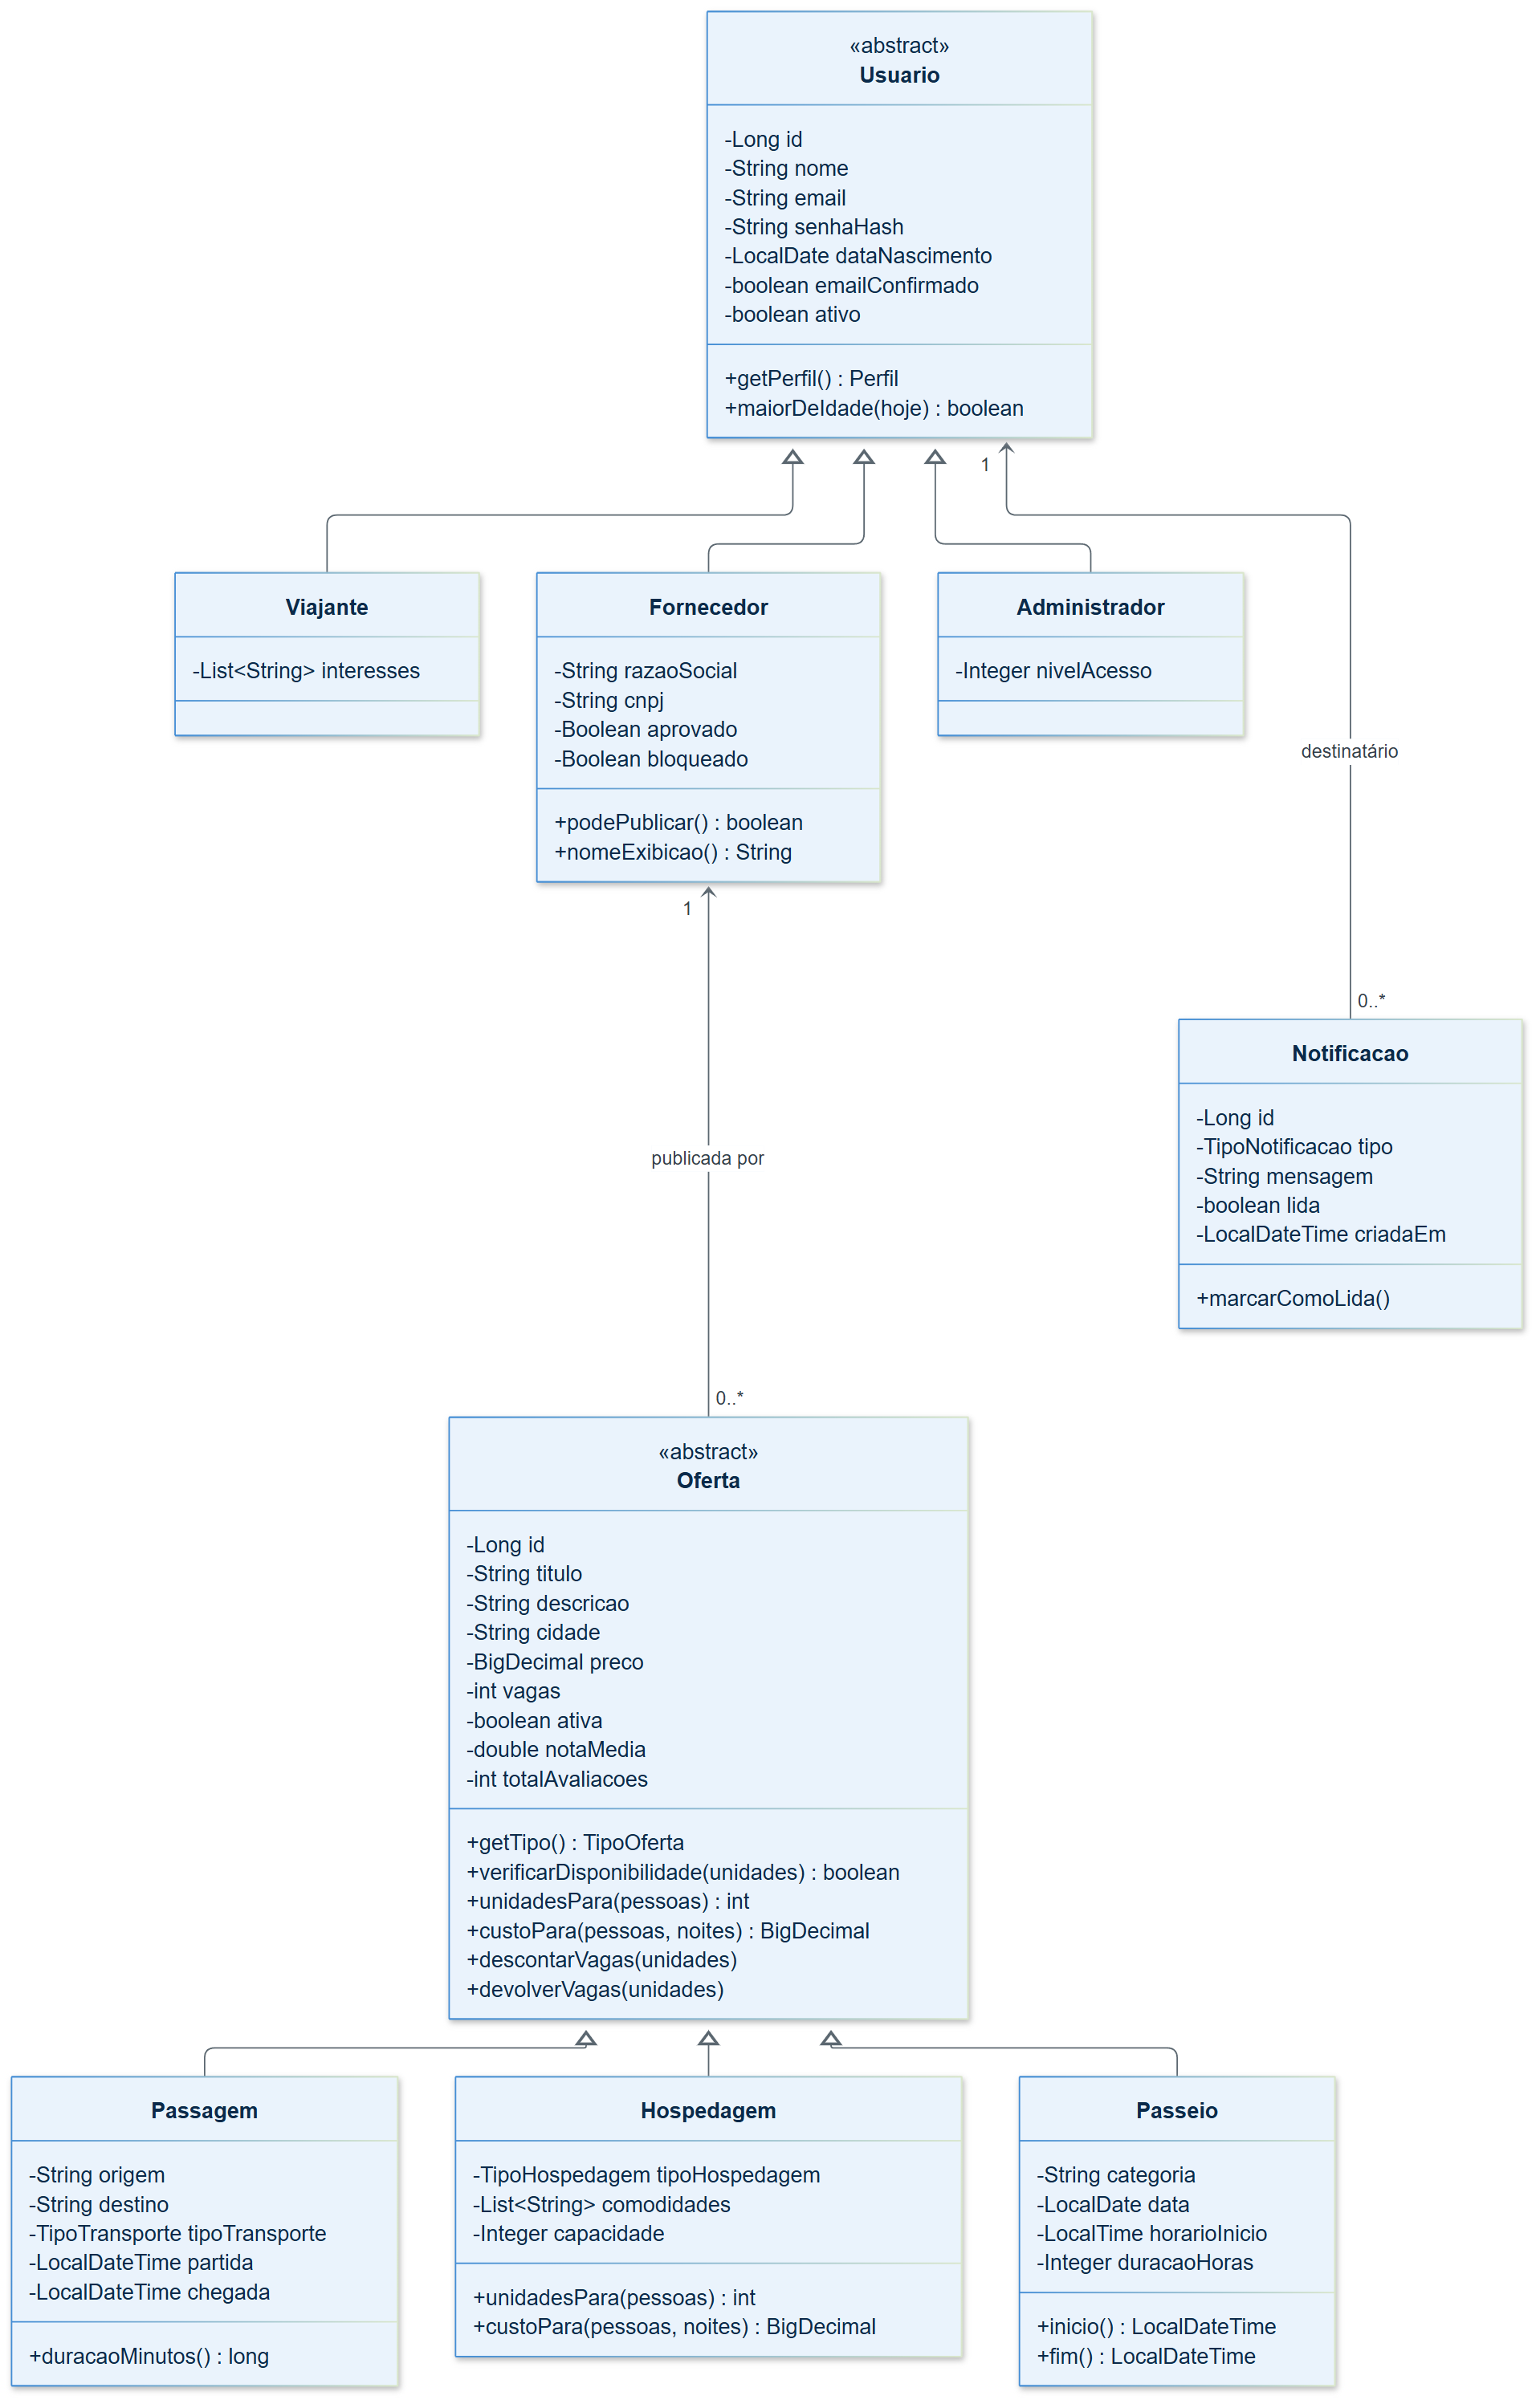
\includegraphics[width=0.82\linewidth,height=0.70\textheight,keepaspectratio]{c4-4-codigo-usuarios-ofertas.png}
    \caption{Classes de usuários e ofertas.}
\end{figure}

\subsection{Itinerário, reserva e avaliação}

\classe{Itinerario} é composto por \classe{ItemItinerario}: apagar o itinerário apaga os itens.
A classe \classe{Reserva} guarda o status e concentra as transições do processo de negócio
(\classe{confirmar}, \classe{recusar}, \classe{expirar} e \classe{cancelar}), junto com as regras de
prazo. O \classe{ValidadorItinerario} devolve a lista de conflitos que bloqueia o envio das
solicitações de reserva.

\begin{figure}[H]
    \centering
    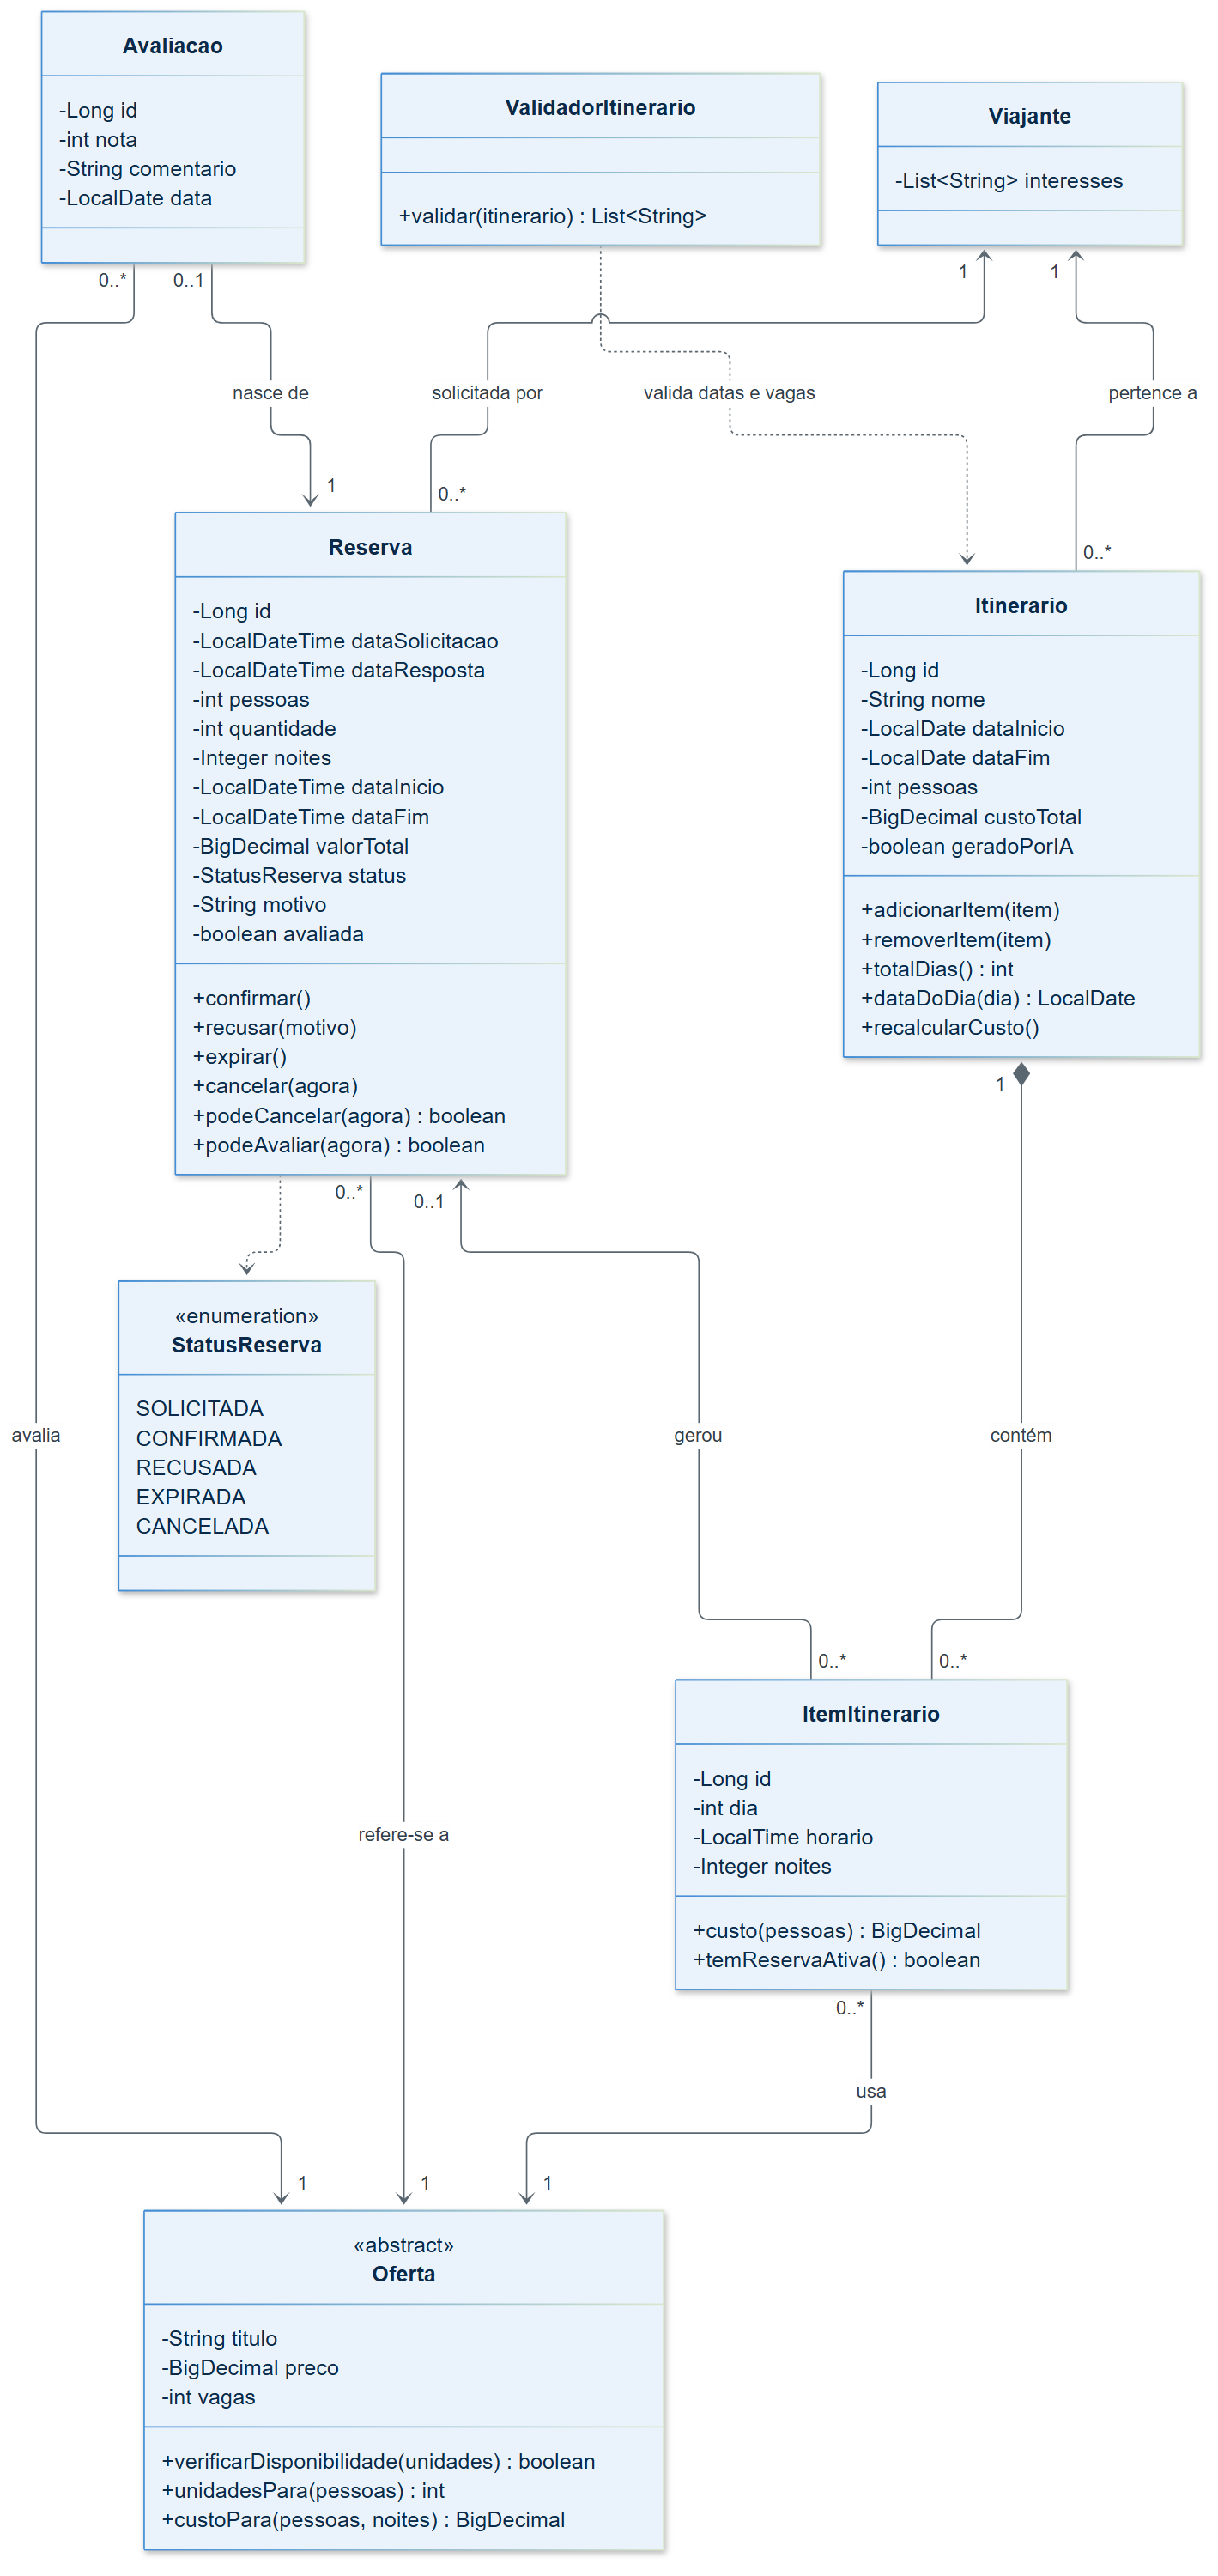
\includegraphics[width=0.62\linewidth,height=0.72\textheight,keepaspectratio]{c4-4-codigo-reservas.png}
    \caption{Classes de itinerário, reserva e avaliação.}
\end{figure}

\subsection{Assistente de roteiro com IA}

O \classe{AssistenteIAService} depende da interface \classe{ClienteLLM}, e não do provedor de IA.
Isso permite trocar o modelo de linguagem e testar o assistente sem chamar a API externa. Os registros
\classe{Candidatos}, \classe{Escolha}, \classe{Janela} e \classe{Plano} representam os passos do
assistente: buscar as ofertas ativas, receber a escolha da IA, validar e montar o roteiro.

\begin{figure}[H]
    \centering
    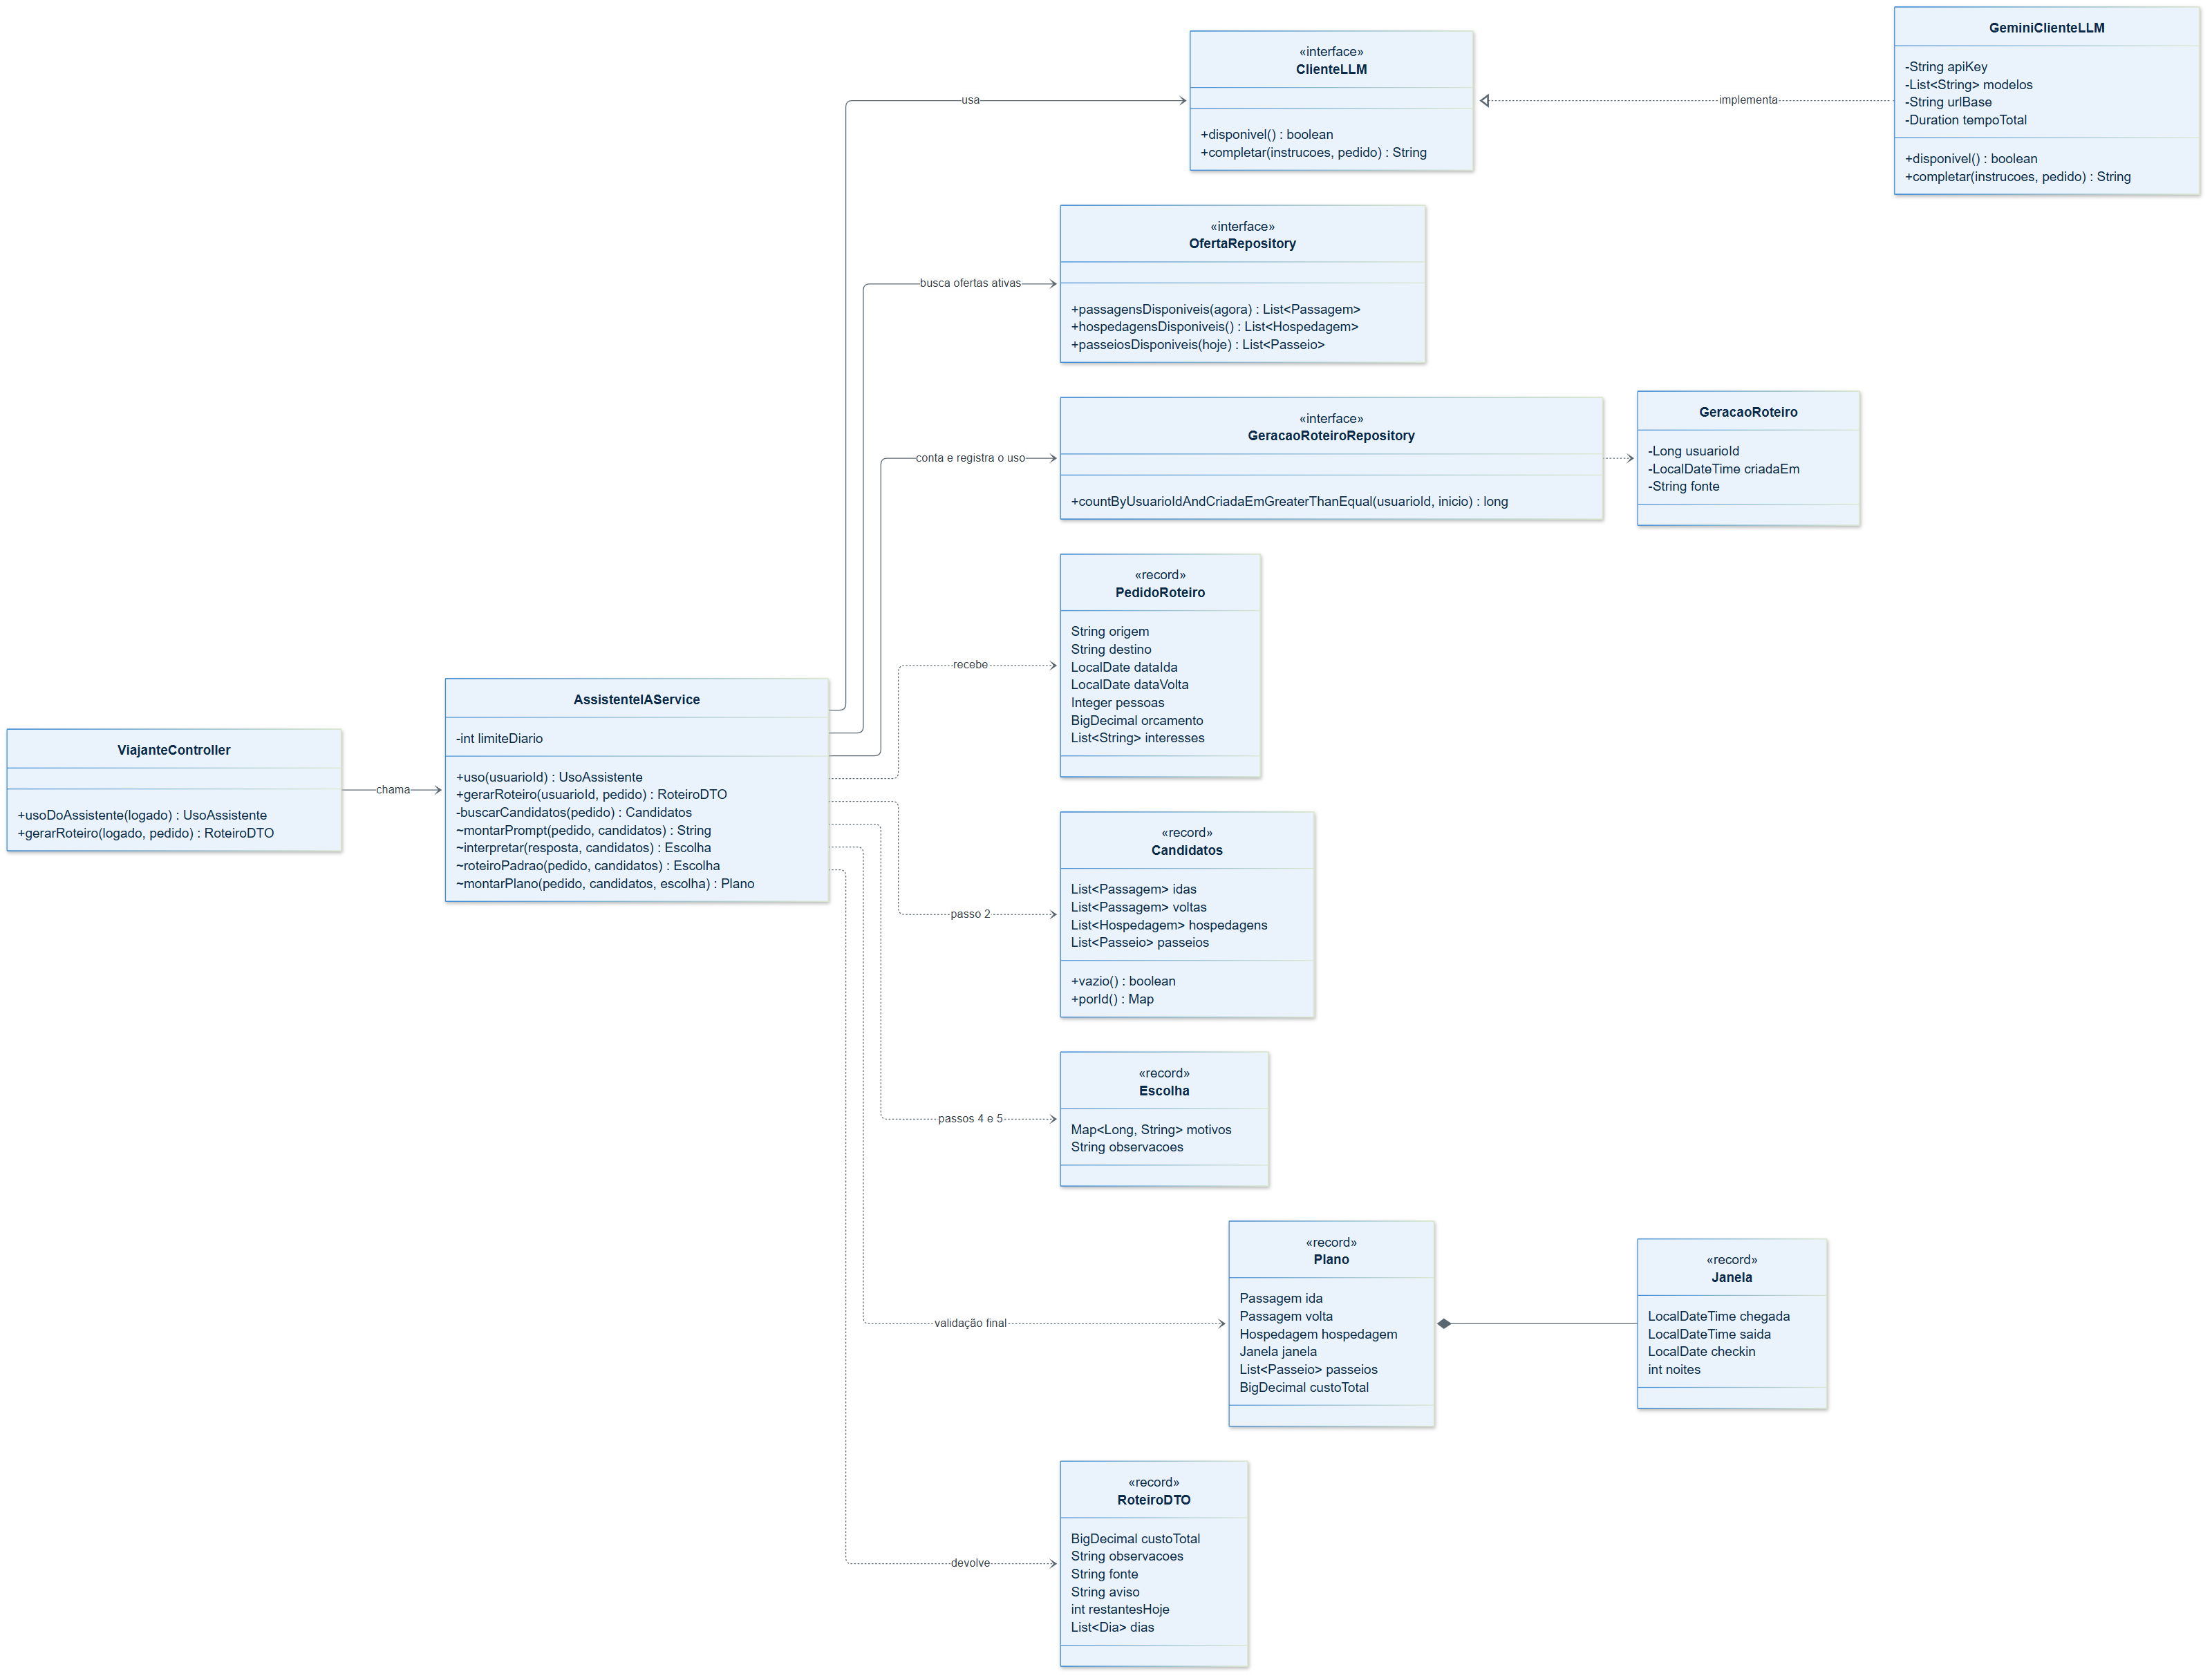
\includegraphics[width=\linewidth,height=0.60\textheight,keepaspectratio]{c4-4-codigo-assistente.png}
    \caption{Classes do assistente de roteiro com IA.}
\end{figure}

\end{document}
